\section{Результаты}
Имплементация описанного выше решения была написана на C++20 с использованием библиотек Assimp, EnTT, fmt, GLFW, GLM, glslang, magic-enum, stb-image, taskflow, VMA, volk, yaml-cpp. Исходный код имеет размер порядка 12 000 строк (не учитывая шейдерный код) и доступен по ссылке \url{https://github.com/tralf-strues/liger-engine}. В качестве тестовых моделей были выбраны сцена Sponza Atrium \cite{sponza_atrium} и меш Medieval Brazier \cite{medieval_brazier} с максимально возможным разрешением текстур.

В следующей таблице приведен анализ одного кадра тестового приложения. Замеры были произведены на компьютере с центральным процессором Intel Core i7-9750H (2.6Ghz) и видеокартой NVIDIA GeForce GTX 1660 Ti (Max-Q Design) при разрешении изображения 1920x1080 пикселей и MSAAx8. Для получения метрик использовался профилировщик NVIDIA Nsight Graphics \cite{nsight}.

\begin{table}[ht]
    \centering
    \begin{tabular}{ p{70mm} | p{30mm} }
    \textbf{Показатель} & \textbf{Значение} \\
    \hline
    \hline
    Меши: instances total & 115 \\
    Меши: instances passed culling & 81 \\
    Меши: triangles total & 3 781 554 \\
    Меши: triangles passed culling & 3 318 486 \\
    \hline
    Кол-во источников света & 28 \\
    Сред. кол-во источников / кластер & 1.53 \\
    Макс. кол-во источников / кластер & 6 \\
    \hline
    \hline
    Clustered Light Cull время & 0.9 мс \\
    \hline
    Particle Emit время & 0.1 мс \\
    Particle Update время & 0.12 мс \\
    Particle Render время & 0.12 мс \\
    \hline
    Mesh Frustum Cull время & <0.01 мс \\
    Mesh Render время & 3.11 мс \\
    \hline
    Bloom время & 0.4 мс \\
    Tone mapping время & 0.07 мс \\
    \hline
    \hline
    Время кадра, мс & 5.2 мс \\
    FPS (кадры в секунду) & 192 \\
    \end{tabular}
    \caption{Анализ одного кадра исполнения тестового приложения.}
    \label{tbl:frame_stats}
\end{table}

Визуализация (без подробной информации, такой как барьеры и параметры ресурсов) кадрового графа реализованного рендерера, сгенерированная собственным отладочным модулем, представлена на рисунке \ref{fig:res_rg_basic}. Более детальная визуализации слишком большая для размещения в данной работе.

\begin{figure}[h]
    \centering
    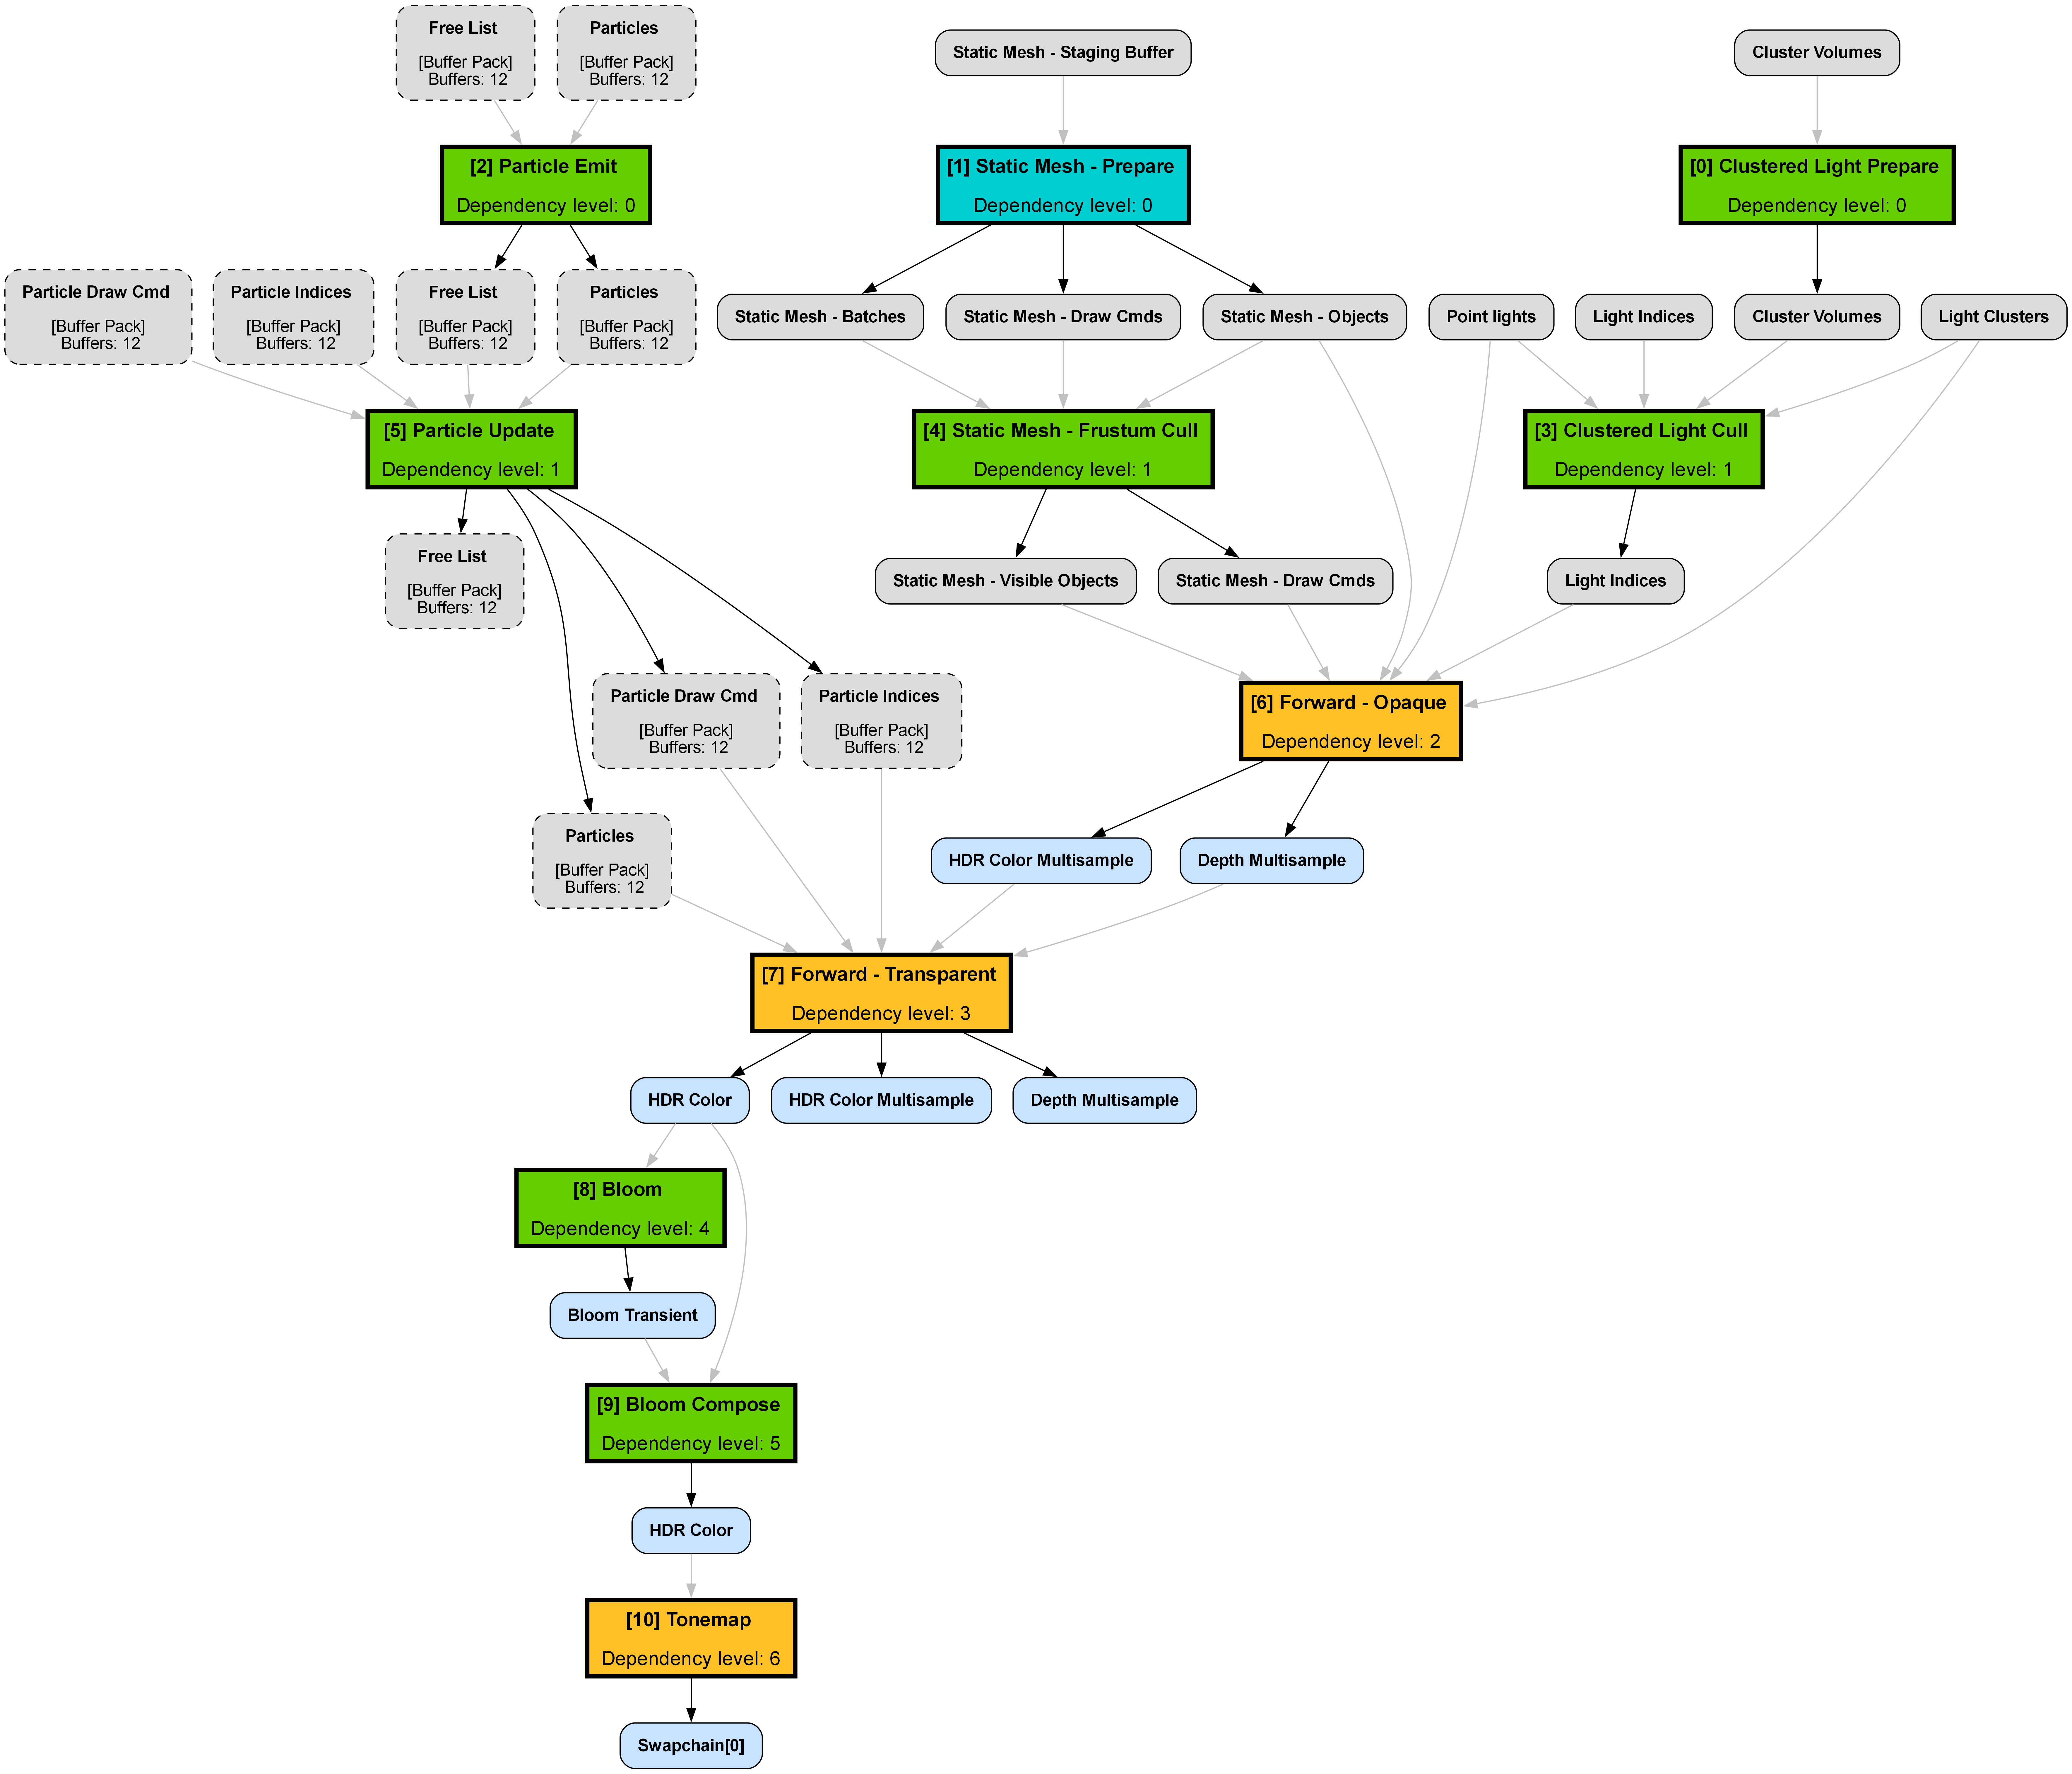
\includegraphics[scale=0.066]{renderer/rg_basic.png}
    \caption{Кадровый граф рендерера, представленного в данной работе.}
    \label{fig:res_rg_basic}
\end{figure}